% $Header: /home/vedranm/bitbucket/beamer/solutions/generic-talks/generic-ornate-15min-45min.en.tex,v 90e850259b8b 2007/0\frac{1}{2}8 20:48:30 tantau $
\documentclass{beamer}
%\documentclass[handout]{beamer}
\usefonttheme[onlymath]{serif}
% This file is a solution template for:
\usepackage{algcompatible}
\usepackage{algpseudocode}
\usepackage{multicol}
% - Giving a talk on some subject.
% - The talk is between 15min and 45min long.
% - Style is ornate.



% Copyright 2004 by Till Tantau <tantau@users.sourceforge.net>.
%
% In principle, this file can be redistributed and/or modified under
% the terms of the GNU Public License, version 2.
%
% However, this file is supposed to be a template to be modified
% for your own needs. For this reason, if you use this file as a
% template and not specifically distribute it as part of a another
% package/program, I grant the extra permission to freely copy and
% modify this file as you see fit and even to delete this copyright
% notice. 

\mode<presentation>
{
  \usetheme{Warsaw}
  % or ...

  \setbeamercovered{transparent}
  % or whatever (possibly just delete it)
}
\setbeamertemplate{navigation symbols}{} 

\usepackage[english]{babel}
% or whatever

\usepackage[latin1]{inputenc}
% or whatever
\useoutertheme{default}

\usepackage{times}
\usepackage[T1]{fontenc}
% Or whatever. Note that the encoding and the font should match. If T1
% does not look nice, try deleting the line with the fontenc.
\newcommand{\beforeverb}{\footnotesize}
\newcommand{\afterverb}{\normalsize}

\title[Solving Classical Equations of Motion] % (optional, use only with long paper titles)
{Lecture 12}

\subtitle
{Solving Classical Equations of Motion} % (optional)

\author[Ying-Jer Kao] % (optional, use only with lots of authors)
{Ying-Jer Kao}
% - Use the \inst{?} command only if the authors have different
%   affiliation.

\institute[National Taiwan University] % (optional, but mostly needed)
{
  Department of Physics\\
 National Taiwan University
  }
% - Use the \inst command only if there are several affiliations.
% - Keep it simple, no one is interested in your street address.

\date[Numerical Analysis and Programming] % (optional)
{\today}

\subject{Talks}
% This is only inserted into the PDF information catalog. Can be left
% out. 



% If you have a file called "university-logo-filename.xxx", where xxx
% is a graphic format that can be processed by latex or pdflatex,
% resp., then you can add a logo as follows:

% \pgfdeclareimage[height=0.5cm]{university-logo}{university-logo-filename}
% \logo{\pgfuseimage{university-logo}}



% Delete this, if you do not want the table of contents to pop up at
% the beginning of each subsection:
%\AtBeginSubsection[]
%{
%  \begin{frame}<beamer>{Outline}
%    \tableofcontents[currentsection,currentsubsection]
%  \end{frame}
%}


% If you wish to uncover everything in a step-wise fashion, uncomment
% the following command: 

%\beamerdefaultoverlayspecification{<+->}


\begin{document}

\begin{frame}
  \titlepage
\end{frame}

\begin{frame}{Outline}
  \tableofcontents
  % You might wish to add the option [pausesections]
\end{frame}


% Since this a solution template for a generic talk, very little can
% be said about how it should be structured. However, the talk length
% of between 15min and 45min and the theme suggest that you stick to
% the following rules:  

% - Exactly two or three sections (other than the summary).
% - At *most* three subsections per section.
% - Talk about 30s to 2min per frame. So there should be between about
%   15 and 30 frames, all told.
\section[Introduction]{Introduction}
\begin{frame}{Introduction}
\begin{itemize}
\item In this lecture, we will discuss the numerical solution of 
ordinary differential equations (ODEs) in classical mechanics.
\item Newton's equation of motion govern the dynamics of:
\begin{itemize}
\item \alert{celestial bodies} in the solar system
\item ``everyday motion'': projectiles, baseballs, mechanical machines
\item  non-electronic aspects of solids, liquids and gases
\end{itemize} 
We will discuss basic numerical algorithms (discretized time axis)
\begin{itemize}
\item 1D equation, properties of different integrators
\item 2D motion, driving forces, disspation...
\end{itemize}
\end{itemize}
\end{frame}

\begin{frame}{1D motion}
\begin{itemize}
\item The simplest case is the 1D motion of a particle with mass $m$ and position $x(t)$.
\item Velocity and acceleration are defined as
\[
\dot{x}(t)=\frac{d x(t)}{d t}=v(t), \quad \ddot{x}(t)=\frac{d^2 x(t)}{d t^2}=a(t)
\]
\item Given a force $F(t)$, Newton's equation of motion is
\[ 
\ddot{x}(t)=\frac{1}{m} F(x(t), \dot{x}(t),t), 
\]
given the initial conditions $x(0)=x_0$ and $v(0)=v_0$.
\end{itemize}
\end{frame}

\begin{frame}{Euler's method}
  \begin{itemize}
    \item The simplest numerical algorithm is Euler's method:
    \item Given the initial conditions $x(0)=x_0$ and $v(0)=v_0$, we can update the position and velocity at each time step $\Delta_t$:
    \begin{align*}
      x(t+\Delta_t) &= x(t)+v(t)\Delta_t,\\
      v(t+\Delta_t) &= v(t)+a(t)\Delta_t.
    \end{align*}
    \item In this case, we update the position and velocity at the same time step.
    \item The algorithm is first-order accurate. The Euler algorithm is not very good in practice and  should not be used in any serious work.
  \end{itemize}
\end{frame}
\begin{frame}{Simple Harmonic Oscillator}
\centerline{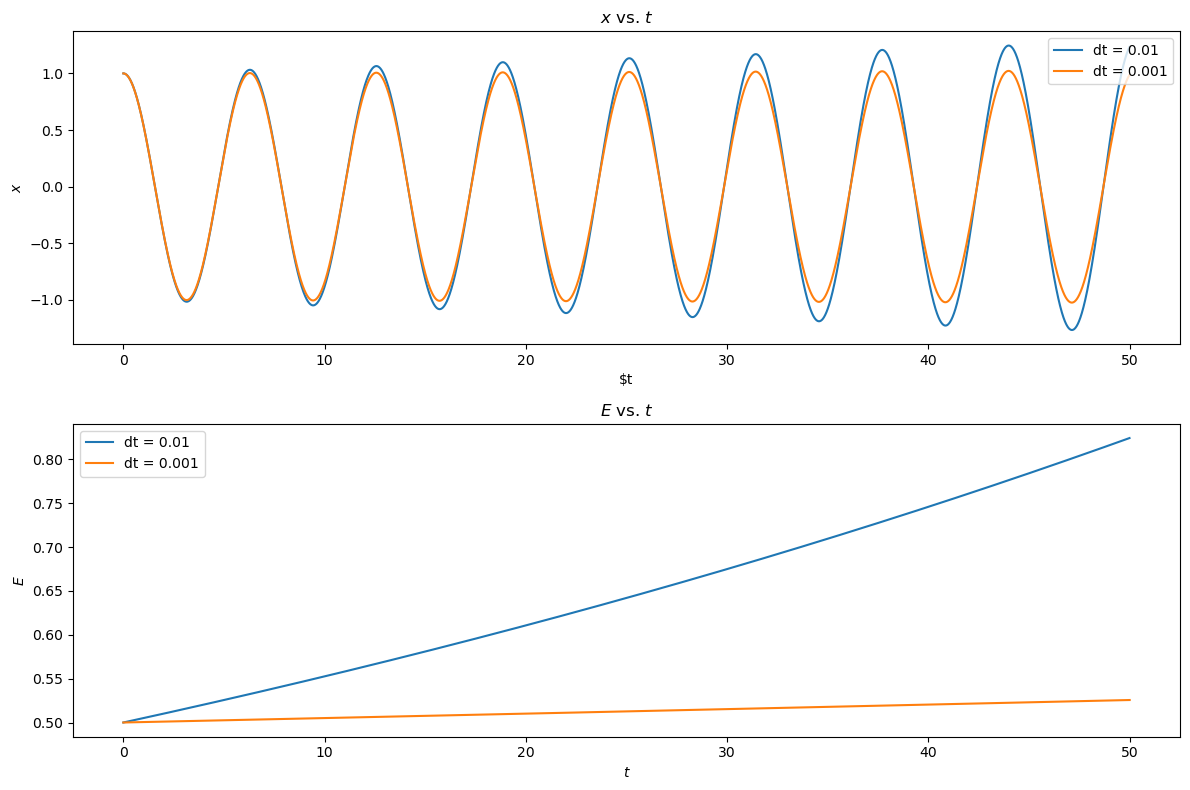
\includegraphics[width=0.8\textwidth]{./eulercmp.png}}
\begin{itemize}
  \item Amplitude increases with time. Unbounded energy error.
  \item We need algorithms with bounded energy error for periodic motion.
\end{itemize}
\end{frame}
\begin{frame}{Leapfrog Method}
  \begin{itemize}
    \item The second-order form of $x$,
    $$
    x_{n+1}=x_n+\Delta_t v_n+\frac{1}{2} \Delta_t^2 a_n+O\left(\Delta_t^3\right)
    $$
\item The first-order form of ${v}$ :
    $$
    v_{n+1}=v_n+\Delta_t a_n+O\left(\Delta_t^2\right)
    $$
\item
    Re-write $x$ formula as
    $$
    x_{n+1}=x_n+\Delta_t\left(v_n+\frac{1}{2} \Delta_t a_n\right)+O\left(\Delta_t^3\right)
    $$
    where we can identify "half-step" velocity 
    \begin{align*}
    v_{n+\frac{1}{2}}&=v_n+\frac{1}{2} \Delta_t a_n+O\left(\Delta_t^2\right)\\
    x_{n+1}&=x_n+\Delta_t v_{n+\frac{1}{2}}+O\left(\Delta_t^3\right)
    \end{align*}
    \item We will only have $v$ on the half-step, use $v_{n-\frac{1}{2}}$ to obtain $v_{n+\frac{1}{2}}$
   $$ 
      v_{n+\frac{1}{2}}  =v_{n-\frac{1}{2}}+\Delta_t a_n, \quad x_{n+1}  =x_n+\Delta_t v_{n+\frac{1}{2}}
   $$ 
  \end{itemize}
\end{frame}
\begin{frame}{Leapfrog Method}

  \begin{itemize}
    \item The leapfrog method is a second-order algorithm: 
    Given the initial conditions $x(0)=x_0$ and $v(0)=v_0$, we can update the position and velocity at each time step $\Delta_t$:
    \begin{align*}
      v(t+\Delta_t/2) &= v(t)+a(t)\Delta_t/2,\\
      x(t+\Delta_t) &= x(t)+v(t+\Delta_t/2)\Delta_t,\\
      v(t+\Delta_t) &= v(t+\Delta_t/2)+a(t+\Delta_t)\Delta_t/2.
    \end{align*}
  \end{itemize}
  \centerline{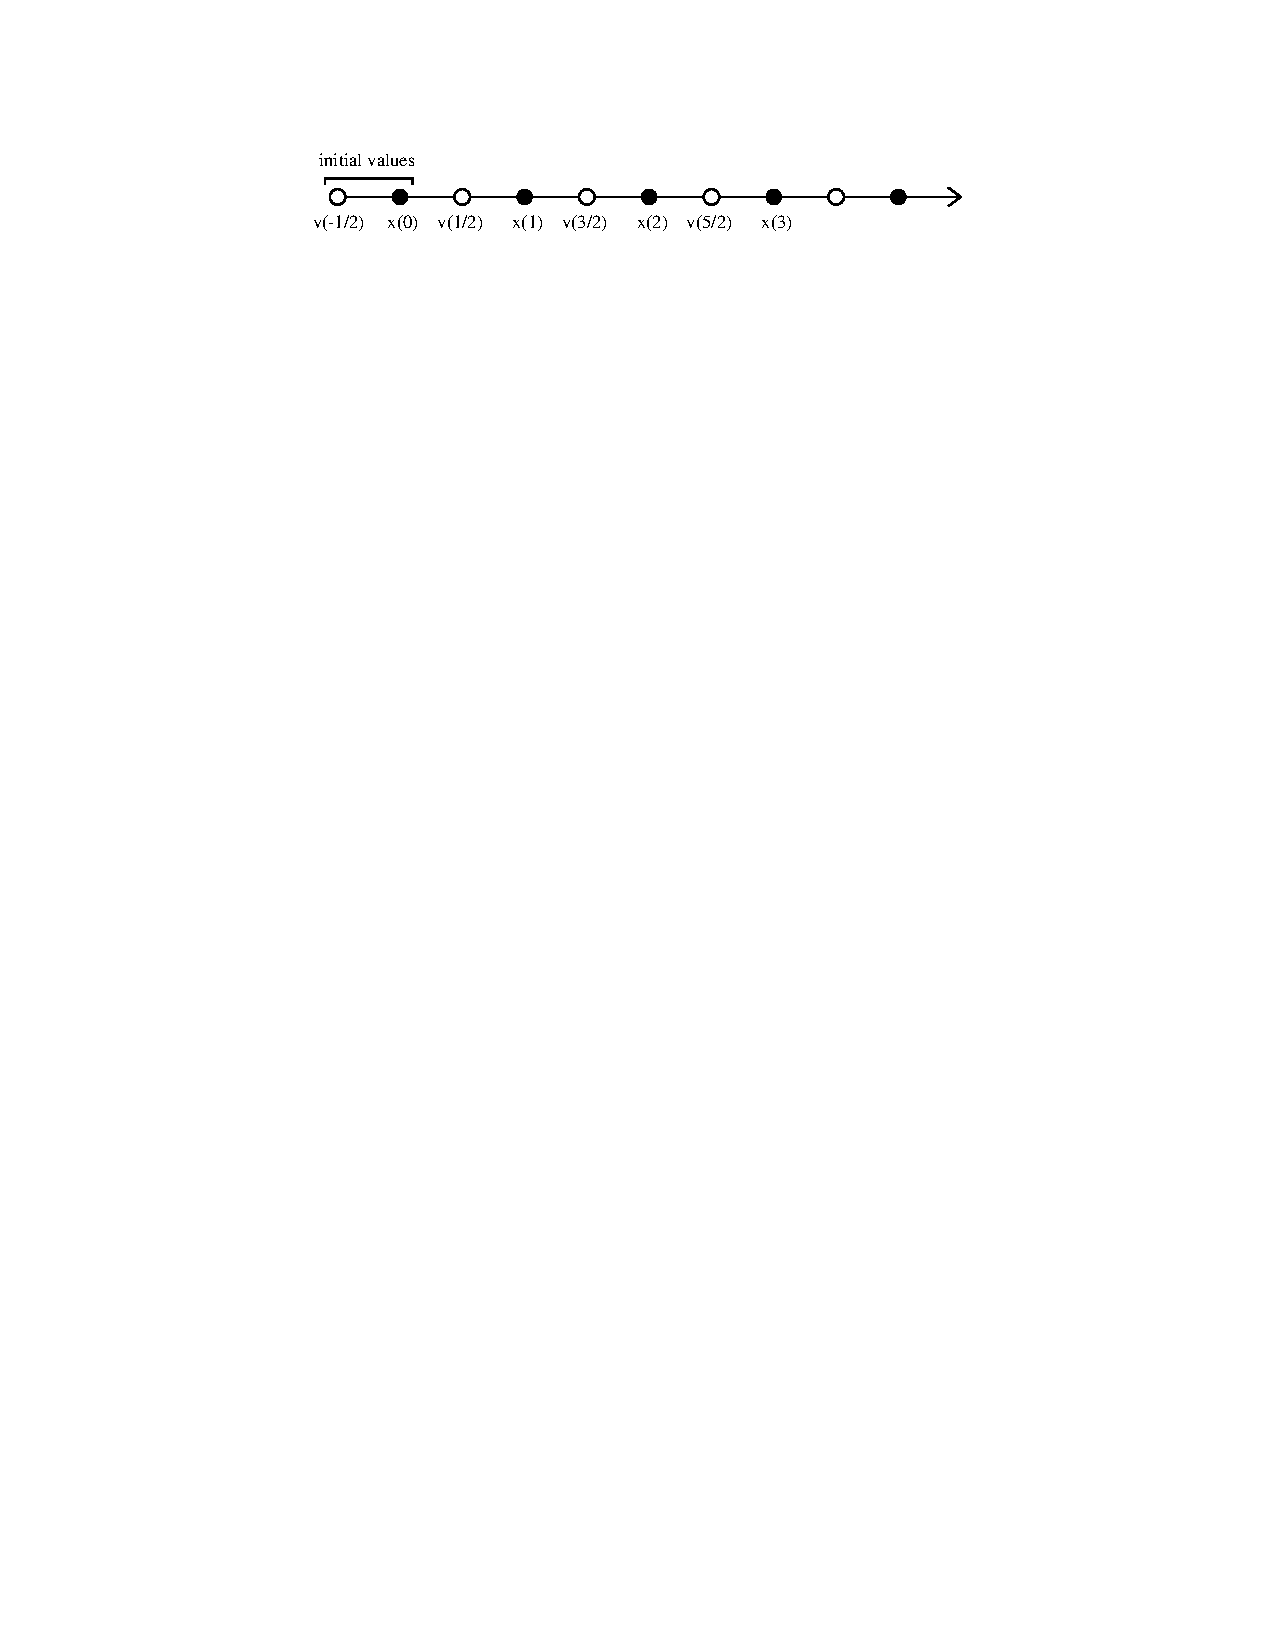
\includegraphics[width=0.8\textwidth]{./leapfrog.pdf}}
\end{frame}
\begin{frame}{Error Estimates}
  \begin{itemize}
    \item The leapfrog method is second-order accurate in time.
    \item The error in the position is $O(\Delta_t^2)$.
    \item The error in the velocity is $O(\Delta_t)$.
    \item The energy error is $O(\Delta_t^2)$.
    \item The leapfrog method is a symplectic integrator, which means that it conserves energy.
    
  \end{itemize}
\end{frame}
\begin{frame}
  \begin{itemize}
    \item Forward and backward $x$ steps 
    \beforeverb
    \begin{align*} 
      & x_{n+1}=x_n+\Delta_t v_n+\frac{1}{2} \Delta_t^2 a_n+\frac{1}{6} 
      \Delta_t^3 \dot{a}_n+O\left(\Delta_t^4\right) \\ 
     +) \quad & x_{n-1}=x_n-\Delta_t v_n+\frac{1}{2} \Delta_t^2 a_n-\frac{1}{6} 
      \Delta_t^3 \dot{a}_n+O\left(\Delta_t^4\right)  
    \end{align*}
    \afterverb
    $\Rightarrow\quad   x_{n+1}=2 x_n-x_{n-1}+\Delta_t^2 a_n+O\left(\Delta_t^4\right)$
    \item Consider
    \beforeverb
    \begin{align*}
     & x_n-x_{n-1}=x\left(t_{n-\frac{1}{2}}+\frac{\Delta_t}{2}\right)-x\left(t_{n-\frac{1}{2}}-\frac{\Delta_t}{2}\right) \\
      &= \left[x_{n-\frac{1}{2}}+\left(\frac{\Delta_t}{2}\right) v_{n-\frac{1}{2}}+\frac{1}{2}\left(\frac{\Delta_t}{2}\right)^2 a_{n-\frac{1}{2}}+\frac{1}{6}\left(\frac{\Delta_t}{2}\right)^3 \dot{a}_{n-\frac{1}{2}}+\ldots\right]  \\
      & \quad-\left[x_{n-\frac{1}{2}}-\left(\frac{\Delta_t}{2}\right) v_{n-\frac{1}{2}}+\frac{1}{2}\left(\frac{\Delta_t}{2}\right)^2 a_{n-\frac{1}{2}}-\frac{1}{6}\left(\frac{\Delta_t}{2}\right)^3 \dot{a}_{n-\frac{1}{2}}+\ldots\right] \\
      &= \Delta_t v_{n-\frac{1}{2}}+O\left(\Delta_t^3\right) 
      \end{align*}
   \afterverb
   
   $ \Rightarrow \quad x_n-x_{n-1}=v_{n-\frac{1}{2}} \Delta_t+O\left(\Delta_t^3\right)$ 
    \end{itemize}
\end{frame}
\begin{frame}
  \begin{itemize}
    \item We have 
    \begin{align*}
      & x_{n+1}=2 x_n-x_{n-1}+\Delta_t^2 a_n+O\left(\Delta_t^4\right) \\
      & x_n-x_{n-1}=v_{n-\frac{1}{2}} \Delta_t+O\left(\Delta_t^3\right) \\
      & x_{n+1}=x_n+\Delta_t\left(v_{n-\frac{1}{2}}+\Delta_t a_n\right)\\
      \Rightarrow \quad & 
          v_{n-\frac{1}{2}}=\frac{1}{\Delta_t}\left(x_n-x_{n-1}\right)+O\left(\Delta_t^2\right) \\
          & x_{n+1}=x_n+\Delta_t\left(v_{n-\frac{1}{2}}+\Delta_t a_n\right)
    \end{align*}
    \item The error in each local update $x_{n+1}$ is  $O(\Delta_t^3)$. 
    \item However, $v_{n+\frac{1}{2}}=v_{n-\frac{1}{2}}+a_n \Delta_t+O\left(\Delta_t^3\right)$, 
    so the erorr in $x$ is $O\left(\Delta_t^4\right)$
  \end{itemize}
\end{frame}
\end{document}


